\documentclass[
            a4paper
            ]{scrartcl}%article

%\usepackage[biber]{assignment}
%\addbibresource{references.bib}
\usepackage{assignment}
\usepackage{amsmath}

\title{Praktisches Übungsbeispiel SS2014}
\subtitle{Zuverlässigkeitsmodellierung}
%\rohead{Übungsbeispiel SS14}
\subject{VU Dependable Systems 182.712}

\author{
 \authorname{Markus Kessler} \\
 \studentnumber{1225380} \\
 \curriculum{033 535}\\
 \email{e1225380@student.tuwien.ac.at}\\\\
 \authorname{Mathias Lechner} \\
 \studentnumber{1225134} \\
 \curriculum{033 535}\\
 \email{e1225134@student.tuwien.ac.at}\\\\
 \authorname{Martin Wührer} \\
 \studentnumber{1225177} \\
 \curriculum{033 535}\\
 \email{e1225177@student.tuwien.ac.at}
}

%\lohead{Kessler, Lechner, Wührer}


\begin{filecontents}{DataTable.dat}
x                        y                        labela                   labelb
1.416197036356566059e+02 5.144315570548267715e+03 7.000000000000000000e+00 1.000000000000000000e+00
2.416197036356566059e+02 3.144315570548267715e+03 8.000000000000000000e+00 4.000000000000000000e+00
4.416197036356566059e+02 1.144315570548267715e+03 6.000000000000000000e+00 2.000000000000000000e+00
\end{filecontents}


\begin{document}

\renewcommand*{\Frefeqname}{Gleichung}
\renewcommand*{\Freffigname}{Abbildung}

\maketitle

\begin{abstract}
Our task is to create a Markov chain model for simulating the failure of a computer system. The mean time to failure and the availability of a simple and a redundant version of the system are compared. Additionally a cost evaluation between the more expensive redundant system and simple system is considered.
\end{abstract}

\section{Executive Summary}

\newpage


\section{Problemstellung}
\begin{figure}
    \centering
    \begin{subfigure}[b]{0.48\linewidth}
    \centering
    \scalebox{.85}{
    \begin{tikzpicture}
        \tikzstyle{node} = [top color=white, bottom color=blue!30, 
                                draw=blue!50!black!100, drop shadow]
        \tikzstyle{switch} = [top color=white, bottom color=red!30, 
                                draw=red!50!black!100, drop shadow,
                                rounded corners=5pt]
        \node[switch](sw1){Switch};
        \node[node] (nd1)   [above left=of sw1]{Node 1};
        \node[node] (nd2)   [above=of sw1]{Node 2};
        \node[node] (nd3)   [above right=of sw1]{Node 3};

        \path (sw1) edge (nd1);
        \path (sw1) edge (nd2);
        \path (sw1) edge (nd3);
    \end{tikzpicture}}
    \caption{Einfache Variante}
    \end{subfigure}
    \begin{subfigure}[b]{0.48\linewidth}
    \scalebox{.85}{
    \begin{tikzpicture}
        \tikzstyle{node} = [top color=white, bottom color=blue!30, 
                                draw=blue!50!black!100, drop shadow]
        \tikzstyle{backup} = [bottom color=green!30]
        \tikzstyle{switch} = [top color=white, bottom color=red!30, 
                                draw=red!50!black!100, drop shadow,
                                rounded corners=5pt]

        \node[switch](sw1){Switch 1};
        \node[switch,backup](sw2)  [right=of sw1]{Switch 2};
        \node[node] (nd1)   [above left=of sw1]{Node 1};
        \node[node] (nd2)   [above=of sw1]{Node 2};
        \node[node] (nd3)   [above=of sw2]{Node 3};
        \node[node,backup] (nd4)   [above right=of sw2]{Node 4};

        \path (sw1) edge (nd1);
        \path (sw1) edge (nd2);
        \path (sw1) edge (nd3);
        \path (sw1) edge (nd4);

        \path (sw2) edge (nd1);
        \path (sw2) edge (nd2);
        \path (sw2) edge (nd3);
        \path (sw2) edge (nd4);
    \end{tikzpicture}}
    \caption{Fehlertolerant erweiterte Variante}
    \end{subfigure}
    \caption{Einfache und fehlertolerant erweiterte Variante des Computersystems}
\end{figure}


\section{Lösungsmethode}
\subsection{MTTF}

\subsubsection{Einfache Variante}

\begin{figure}
    \centering
    \begin{subfigure}[b]{0.48\linewidth}
        \centering
        \begin{tikzpicture}[>=latex]
            \tikzstyle{markov} = [top color=blue!30, bottom color=white, 
                            draw=blue!50!black!100, drop shadow]
            \tikzstyle{bad} = [top color=red!30]

            \node[markov,circle split,label=below left:{\textbf{a}}] (1) {$3/3$ \nodepart{lower} $1/1$};
            \node[markov,bad,circle split,label=below right:{\textbf{b}}] (2) [above right=of 1]{$2/3$ \nodepart{lower} $1/1$};
            \node[markov,bad,circle split,label=below right:{\textbf{c}}] (3) [below right=of 1]{$3/3$ \nodepart{lower} $0/1$};
            \draw[->] (1) to node[sloped,above]{$3\lambda_R$}(2);
            \draw[->] (1) to node[sloped,above]{$\lambda_N$}(3);
        \end{tikzpicture}
        \caption{\textbf{Zustand a}: Funktionierend, \\
            \textbf{Zustand b}: Rechnerausfall, \\
            \textbf{Zustand c}: Netzwerkausfall}
        \label{fig:states_simple_mttf}
    \end{subfigure}
    \begin{subfigure}[b]{0.48\linewidth}
        \centering
            \begin{tikzpicture}[>=latex]
                \tikzstyle{markov} = [top color=blue!30, bottom color=white, 
                                draw=blue!50!black!100, drop shadow]
                \tikzstyle{bad} = [top color=red!30]

                \node[markov,circle,label=below right:{\textbf{a}}] (1) {alive};
                \node[markov,bad,circle,label=below right:{\textbf{b}}] (2)
                [right=5 of 1]{dead};
                \draw[->] (1) to node[sloped,above]{$3\lambda_R + \lambda_N$}(2);
            \end{tikzpicture}
            \caption{Vereinfachte Variante von \Fref{fig:states_simple_mttf} \\
                \textbf{Zustand a}: Funktionierend, \\
                \textbf{Zustand b}: nicht Funktionierend}
            \label{fig:states_simple_mttf_simply}
    \end{subfigure}
    \caption{Zustände Einfache Variante MTTF}
    \label{fig:states_simple_mttf_comb}
\end{figure}

Wir definieren für dieses Modell folgende Zustände (siehe \Fref{fig:states_simple_mttf})
\begin{enumerate}[\bfseries a.]
    \item das System arbeitet fehlerfrei ($3/3$ | $1/1$)
    \item ein Node ist defekt ($2/3$ | $1/1$)
    \item ein Switch ist defekt ($3/3$ | $0/1$)
\end{enumerate}

Da es keine Rolle spielt, ob ein Rechner oder das Netzwerk ausfällt, kann das
Modell vereinfacht werden. Wir sprechen nur noch von "alive" und "dead". (siehe
\Fref{fig:states_simple_mttf_simply})
Die Wahrscheinlichkeiten werden addiert.

\subsubsection{Redundante Variante}
\begin{figure}
    \centering
        \begin{tikzpicture}[>=latex]
            \tikzstyle{markov} = [top color=blue!30, bottom color=white, 
                            draw=blue!50!black!100, drop shadow]
            \tikzstyle{bad} = [top color=red!30]

            \node[markov,circle split,label=below left:{\textbf{a}}] (42) {$4/4$ \nodepart{lower} $2/2$};
            \node[markov,circle split,label=above right:{\textbf{b}}] (32) [above right=of 42]{$3/4$ \nodepart{lower} $2/2$};
            \node[markov,circle split,label=below right:{\textbf{d}}] (31) [below right=of 32]{$3/4$ \nodepart{lower} $1/2$};
            \node[markov,circle split,label=below right:{\textbf{c}}] (41) [below right=of 42]{$4/4$ \nodepart{lower} $1/2$};
            \node[markov,bad,circle,label=below right:{\textbf{e}}] (d)  [right=3 of 31]{dead};
            \draw[->] (42) to node[sloped,above]{$4\lambda_R$}(32);
            \draw[->] (32) to[bend right=45] node[sloped,above]{$\mu_R$}(42);
            \draw[->] (42) to node[sloped,above]{$2\lambda_N$}(41);
            \draw[->] (41) to[bend right=-45] node[sloped,above]{$\mu_N$}(42);
            \draw[->] (41) to node[sloped,above]{$4\lambda_R$}(31);
            \draw[->] (31) to node[sloped,above]{$\mu_N$} (42);
            \draw[->] (32) to node[sloped,above]{$2\lambda_N$}(31);
            \draw[->] (32) to[bend left=20] node[sloped,above]{$3\lambda_R$}(d);
            \draw[->] (31) to node[sloped,above]{$3\lambda_R+\lambda_N$}(d);
            \draw[->] (41) to[bend right=20] node[sloped,above]{$\lambda_N$}(d);
        \end{tikzpicture}
    \caption{Zustände redundante Variante MTTF}
    \label{fig:states_redundant_mttf}
\end{figure}

Für die redundante Variante existieren die Zustände (siehe
\Fref{fig:states_redundant_mttf})
\begin{enumerate}[\bfseries a.]
    \item das System arbeitet fehlerfrei ($4/4$ | $2/2$)
    \item ein Node ist defekt ($3/4$ | $2/2$)
    \item ein Swich ist defekt ($4/4$ | $1/2$)
    \item ein Node sowie ein Switch sind defekt ($3/4$ | $1/1$)
    \item das System ist defekt ("dead")
\end{enumerate}

Für den Fall (\textbf{d}) gehen wir davon aus, dass der Techniker beide Fehler gleichzeitig beheben kann. 
Beispielsweise kommt er mit einem Ersatznode und -switch und tauscht beide aus. 
Deshalb existiert in diesem Modell keine Möglichkeit von (\textbf{d}) auf
(\textbf{c}) oder (\textbf{b}) zu kommen.

\subsection{Availability}
\subsubsection{Einfache Variante}
\begin{figure}
    \centering
    \begin{subfigure}[b]{0.48\linewidth}
        \centering
        \begin{tikzpicture}[>=latex]
            \tikzstyle{markov} = [top color=blue!30, bottom color=white, 
                            draw=blue!50!black!100, drop shadow]
            \tikzstyle{bad} = [top color=red!30]

            \node[markov,circle split,label=below left:{\textbf{a}}] (1) {$3/3$ \nodepart{lower} $1/1$};
            \node[markov,bad,circle split,label=below right:{\textbf{b}}] (2) [above right=of 1]{$2/3$ \nodepart{lower} $1/1$};
            \node[markov,bad,circle split,label=below right:{\textbf{c}}] (3) [below right=of 1]{$3/3$ \nodepart{lower} $0/1$};
            \draw[->] (1) to node[sloped,above]{$3\lambda_R$}(2);
            \draw[->] (1) to node[sloped,above]{$\lambda_N$}(3);
            \draw[->, green!70!black] (3) to[bend right=45] node[sloped,above]{$\mu_N$}(1);
            \draw[->, green!70!black] (2) to[bend right=45] node[sloped,above]{$\mu_R$}(1);
        \end{tikzpicture}
        \caption{\textbf{Zustand a}: Funktionierend, \\
            \textbf{Zustand b}: Rechnerausfall, \\
            \textbf{Zustand c}: Netzwerkausfall}
        \label{fig:states_simple_avail}
    \end{subfigure}
    \begin{subfigure}[b]{0.48\linewidth}
        \centering
            \begin{tikzpicture}[>=latex]
                \tikzstyle{markov} = [top color=blue!30, bottom color=white, 
                                draw=blue!50!black!100, drop shadow]
                \tikzstyle{bad} = [top color=red!30]

                \node[markov,circle,label=below right:{\textbf{a}}] (1) {alive};
                \node[markov,bad,circle,label=below right:{\textbf{b}}] (2)
                [right=5 of 1]{dead};
                \draw[->] (1) to node[sloped,above]{$3\lambda_R + \lambda_N$}(2);
                \draw[->, green!70!black] (2) to[bend right=45] node[sloped,above]{$\mu_R=\mu_N$}(1);
            \end{tikzpicture}
            \caption{Vereinfachte Variante von \Fref{fig:states_simple_avail} \\
                \textbf{Zustand a}: Funktionierend, \\
                \textbf{Zustand b}: nicht Funktionierend}
            \label{fig:states_simple_avail_simply}
    \end{subfigure}
    \caption{Zustände Einfache Variante Availability}
    \label{fig:states_simple_avail_comb}
\end{figure}
Wir übernehmen für die Berechnung der Verfügbarkeit das vorherige Modell,
erweitern es jedoch mit einem Übergang von \enquote{dead} zu \enquote{alive}
(siehe \Fref{fig:states_simple_avail_comb}).

\subsubsection{Redundante Variante}
\begin{figure}
    \centering
        \begin{tikzpicture}[>=latex]
            \tikzstyle{markov} = [top color=blue!30, bottom color=white, 
                            draw=blue!50!black!100, drop shadow]
            \tikzstyle{bad} = [top color=red!30]

            \node[markov,circle split,label=below left:{\textbf{a}}] (42) {$4/4$ \nodepart{lower} $2/2$};
            \node[markov,circle split,label=above right:{\textbf{b}}] (32) [above right=of 42]{$3/4$ \nodepart{lower} $2/2$};
            \node[markov,circle split,label=below right:{\textbf{d}}] (31) [below right=of 32]{$3/4$ \nodepart{lower} $1/2$};
            \node[markov,circle split,label=below right:{\textbf{c}}] (41) [below right=of 42]{$4/4$ \nodepart{lower} $1/2$};
            \node[markov,bad,circle,label=below right:{\textbf{e}}] (d)  [right=3 of 31]{dead};
            \draw[->] (42) to node[sloped,above]{$4\lambda_R$}(32);
            \draw[->] (32) to[bend right=45] node[sloped,above]{$\mu_R$}(42);
            \draw[->] (42) to node[sloped,above]{$2\lambda_N$}(41);
            \draw[->] (41) to[bend right=-45] node[sloped,above]{$\mu_N$}(42);
            \draw[->] (41) to node[sloped,above]{$4\lambda_R$}(31);
            \draw[->] (31) to node[sloped,above]{$\mu_N$} (42);
            \draw[->] (32) to node[sloped,above]{$2\lambda_N$}(31);
            \draw[->] (32) to[bend left=20] node[sloped,above]{$3\lambda_R$}(d);
            \draw[->] (31) to node[sloped,above]{$3\lambda_R+\lambda_N$}(d);
            \draw[->] (41) to[bend right=20] node[sloped,above]{$\lambda_N$}(d);
            \draw[->,green!70!black] (d) to[bend right=108] node[sloped,above]{$\mu_N=\mu_R$}(42);
        \end{tikzpicture}
    \caption{Zustände redundante Variante Availability}
    \label{fig:states_redundant_avail}
\end{figure}
Bei der redundanten Variante fügen wir ebenfalls ein Übergang von \enquote{dead}
zum Startzustand ein. Für die Berechnung der Verfügbarkeit definieren wir, dass
das System nur in den blauen Zuständen verfügbar ist (siehe
\Fref{fig:states_redundant_avail}).

\section{Ergebnisse}
\begin{figure}
\centering
\begin{tikzpicture}
    \begin{axis}[xmin=0, xmax=1800,
        height=5.2cm, width=12cm,
        ymin=0, ymax=1,
        axis lines=center,
        axis on top=true,
        domain=0:1,
        legend style={at={(axis cs:1800,0.2)},anchor=south east},
        %ylabel=Number of failed banks
        ] % use TeX as calculator: 
    \addplot[blue,thick,domain=0:1800,samples=100] table {values_simple_mttf.dat}; 
    \addlegendentry{MTTF ohne Redundanz}
    \addplot[red,thick,domain=0:1800,samples=100] table {values_redundancy_mttf.dat}; 
    \addlegendentry{MTTF mit Redundanz}
    \addplot[green,thick,domain=0:1800,samples=100] table {values_redundancy_without_repair_mttf.dat}; 
    \addlegendentry{-||- ohne Reparatur}
    \end{axis} 
\end{tikzpicture}
\caption{Vergleich der Ausfallwahrscheinlichkeit MTTF}
\label{fig:mttf_result}
\end{figure}
Die Ergebnisse von MTTF sind in \Fref{fig:mttf_result} dargestellt.

\section{Diskussion}
\begin{figure}
\centering
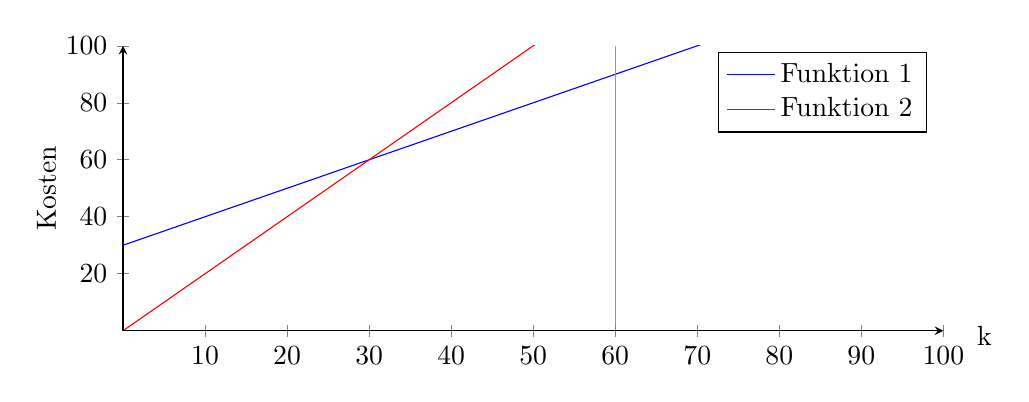
\begin{tikzpicture}
    \begin{axis}[
	    height=5.2cm, width=12cm,
		axis lines=center,
		axis on top=true,
		domain=0:100,
    	xmin=0, xmax=100,
    	xlabel=k,
        ymin=0, ymax=100,
        ylabel=Kosten,
        x label style={at={(axis description cs:1.05,0.05)},anchor=north},
        y label style={at={(axis description cs:-0.07,.5)},rotate=90,anchor=south},
        %ylabel=Number of failed banks
        ] % use TeX as calculator: 
    \addplot +[mark=none]{30+x};
    \addlegendentry{Funktion 1}
    \addplot +[mark=none]{2*x};
    \addlegendentry{Funktion 2}
    \draw[green] ({axis cs:60,0}|-{rel axis cs:0,1}) -- ({axis cs:60,0}|-{rel axis cs:0,0});
    \end{axis} 
\end{tikzpicture}
\caption{Vergleich der Kostenfunktionen mit Schnittpunkt $K_x$}
\label{fig:mttf_result}
\end{figure}
\subsection{Kostenrechnung}
Aus der Simulation mit \emph{SHARPE} haben wir die beiden Availability Werte $\alpha_s$ (für das einfache System) und $\alpha_r$ für das Redundante System erhalten.\\
Sei $\Omega$ die Betriebskosten des einfachen Systems, so lassen sich die Kosten beschreiben mit:
\begin{equation}
C_s(k) = \Omega \cdot \alpha_s + (1-\alpha_s)\Omega \cdot k
\end{equation}

wobei $k \cdot \Omega$ die Ausfallkosten des Systems sind ($k \in \mathbb{N}^+$)\\$k$ stellt das Verhältnis zwischen Laufender Kosten und Ausfallkosten des einfachen Systems dar.\\
Die Kosten des Redundanten Systems ergeben sich mit: 
\begin{equation}
C_r(k) = \Omega \cdot 2,5 \alpha_r + (1- \alpha_r) \cdot \Omega \cdot k
\end{equation}

Um das Verhältnis $k$ zu bestimmen, ab dem sich der Betrieb des Redundanten Systems auszahlt, muss der Schnittpunkt $k_x$ bestimmt werden:
\begin{equation}
\begin{split}
C_s(k_x) = C_r(k_x) \\ &
 \Leftrightarrow
\Omega \cdot \alpha_s + (1-\alpha_s)\Omega \cdot k_x = \Omega \cdot 2,5 \alpha_r + (1- \alpha_r) \cdot \Omega \cdot k_x \\ & \Leftrightarrow
k_x \cdot (1 - \alpha_s - 1 + \alpha_r) = 2,5 \alpha_r - \alpha_s \\ & \Leftrightarrow
k_x = \frac{2,5 \alpha_r - \alpha_s}{\alpha_r - \alpha_s}
\end{split}
\end{equation}
\section{Fazit}
\newpage
\appendix
\section{Sharpe-Quellcode}
\subsection{MTTF}
\subsubsection{MTTF Ohne Redundanz}
\lstinputlisting{simple_mttf.shp}
\subsubsection{MTTF mit Redundanz inklusive Reparatur}
\lstinputlisting{redundancy_mttf.shp}
\subsubsection{MTTF mit Redundanz ohne Reparatur}
\lstinputlisting{redundancy_without_repair_mttf.shp}
\subsection{Availability}
\subsubsection{Availability Ohne Redundanz}
\lstinputlisting{simple_availibility.shp}
\subsubsection{Availability mit Redundanz}
\lstinputlisting{redundant_availability.shp}
\end{document}
